\section{First Experimental Tests}

In polarized deep inelastic scattering, a longitudinally polarized lepton beam
is scattered off of nucleon targets polarized parallel or perpendicular to the
beam axis. Asymmetries are formed by comparing event rates for scattering in
different spin configurations. For a spin $\frac{1}{2}$ target, the
asymmetries of interest are

% Stiegler 2.3 is useful here

\begin{equation}
  A_{\parallel} = \frac{\sigma^{\rightarrow \Leftarrow} - \sigma^{\rightarrow \Rightarrow}}{\sigma^{\rightarrow \Leftarrow} + \sigma^{\rightarrow \Rightarrow}}, ~~~~~~~
  A_{\perp} = \frac{\sigma^{\rightarrow \Uparrow} - \sigma^{\rightarrow \Downarrow}}{\sigma^{\rightarrow \Uparrow} + \sigma^{\rightarrow \Downarrow}}
\end{equation}

Spin-dependent cross sections can be calculated by contracting the elastic
Compton amplitude $T_{\mu \nu}$ with the photon polarization vectors; in the
presence of parity conservation and time reversal, four of these are
independent \cite{}:
%
\begin{eqnarray}
  \sigma_{1/2} & = & F_1 + g_1 - \gamma^2 g_2, \nonumber \\
  \sigma_{3/2} & = & F_1 - g_1 + \gamma^2 g_2, \nonumber \\
  \sigma_L & = & -F_1 + F_2(1+\gamma^2)/(2x),  \nonumber \\
  \sigma_{TL} & = & \sqrt{2}\gamma (g_1+g_2).
\end{eqnarray}
%
Here $\gamma^2 = Q^2/v^2$. These four cross sections are commonly rearranged
into a pair of virtual photon asymmetries $A_1$ and $A_2$:
%
\begin{equation}
  A_1 = \frac{\sigma_{1/2} - \sigma_{3/2}}{\sigma_{1/2} + \sigma_{3/2}}, ~~~~ A_2 = \frac{\sigma_{TL}}{\sigma_T}
\end{equation}
%
The longitudinal and transverse DIS asymmetries can then be written in terms
of these virtual photon asymmetries. In the case of $A_{\parallel}$ we have
\begin{equation}
  A_{\parallel} = D(A_1 + \eta A_2),
\end{equation}
%
where the coefficients $D$ and $\eta$ can be approximated to first order in
$\gamma$ in terms of the usual DIS kinematic variables and $R =
\frac{\sigma_{L}}{\sigma_T}$:
% Detailed derivation of these results can be found in \cite{Anselmino:1994gn}
\begin{equation}
  D \approx \frac{y(2-y)}{y^2 + 2(1-y)(1+R)}, ~~~~~~~~ \eta \approx \frac{2(1-y)}{y(2-y)} \frac{\sqrt{Q^2}}{E}.
\end{equation}
%
Similar equations exist for $A_{\perp}$, such that a measurement of both
asymmetries allows an extraction of both $A_1$ and $A_2$. $D$ can be thought
of as a depolarization factor arising from the fact that the photon is not
fully aligned with the lepton beam, and $\eta$ is a kinematic factor that is
usually small. Finally, the polarized structure functions can be written in
terms of $A_{1,2}$:
\begin{equation}
  g_1 = \frac{F_2}{2x(1+R)}(A_1+\gamma A_2), ~~~~~ g_2 = \frac{F_2}{2x(1+R)}(A_2/\gamma - A_1).
\end{equation}
Thus, measurements of $A_{\parallel}$, $A_{\perp}$, $F_2$, and $R$ are
sufficient to determine the polarized structure functions of the nucleon.

The first DIS experiments to extract $g_1$ using this methodology were E80 and
E130, conducted in the late 1970s and early 1980s at SLAC. These experiments
scattered longitudinally polarized electron beams off of longitudinally
polarized proton targets and measured $A_{\parallel}^p$ in the range $0.1 < x <
0.7$. Using the positivity limit $A_2 < \sqrt{R}$ they determined that
$A_{\parallel}/D$ was a good approximation for $A_1$, and after exploiting that
assumption their results \cite{Alguard:1976bm, Baum:1983ha} were consistent with
expectations from the parton model.
% there are 2-3 more result papers cited in Baum:1983ha if I want them

In 1988, the European Muon Collaboration (EMC) published data on asymmetries of
longitudinally polarized muon beams scattering off of longitudinally polarized
proton targets. The EMC experiment boasted kinematic coverage down to $x =
0.01$, an order of magnitude lower than the earlier SLAC experiments, and the
Collaboration extracted measurements of the proton's $g_1$ structure function
using the same assumption that $A_1 \approx A_{\parallel}/D$. The EMC data on
$A_1$ are consistent with the results from SLAC in their overlapping kinematic
regime, but at low $x$ the EMC results deviate significantly from parton model
predictions. As shown in Figure \ref{fig:emc-g1p}, the value of $\Gamma_1^p$
obtained from the EMC extraction is incompatible with the prediction from Ellis
and Jaffe. Solving for the polarized parton densities using this result and the
beta decay measurements in \ref{eqn:beta-decay}, one finds that the strange
quarks possess a significant polarization antiparallel to the proton, and that
the quark spin contribution to the spin of the proton is only twelve percent:
%
% TODO these numbers come directly from EMC; should do it myself with my beta decay values
\begin{eqnarray}
  \langle S_z \rangle_{u} &=& \frac{1}{2}\left(\Delta u + \Delta \bar{u}\right) = 0.391 \pm 0.016 \pm 0.023, \nonumber \\
  \langle S_z \rangle_{d} &=& \frac{1}{2}\left(\Delta d + \Delta \bar{d}\right) = -0.236 \pm 0.016 \pm 0.023, \nonumber \\
  \langle S_z \rangle_{s} &=& \frac{1}{2}\left(\Delta s + \Delta \bar{s}\right) = -0.095 \pm 0.016 \pm 0.023, \nonumber \\
  \langle S_z \rangle_{quarks} &=& \frac{a_0}{2} = 0.060 \pm 0.047 \pm 0.069.
\end{eqnarray}
%
The EMC result sparked what was once termed a ``spin crisis'' in particle
physics. Successive polarized DIS experiments at CERN, SLAC, and DESY confirmed
and refined the EMC measurement of \(g_1^p\) with improved precision over a
wider kinematic range \cite{Adams:1994zd}, and measured both \(g_1^n\)
\cite{Anthony:1993uf} and \(g_1^d\) \cite{Adeva:1993km} which allowed a
verification of the critical Bjorken sum rule. Over the years the precise value
of \(\Gamma_1^p\) has shifted somewhat, but the implication remains the same ---
the na\"ive parton model cannot explain how the proton gets its spin.

\begin{figure}
  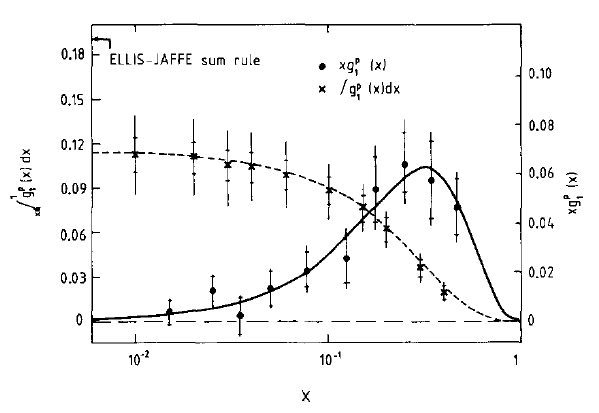
\includegraphics[width=1.0\textwidth]{figures/emc-g1p}
  \caption{EMC extraction of $g^1_p$ and its integral compared to the prediction from Ellis-Jaffe \cite{Ashman:1987hv}}
  \label{fig:emc-g1p}
\end{figure}
